% Search for all the places that say "PUT SOMETHING HERE".

\documentclass[11pt]{article}
\usepackage{amsmath,textcomp,amssymb,geometry,graphicx,enumerate}

\def\Name{Ran Liao}  % Your name
\def\SID{3034504227}  % Your student ID number
\def\Homework{8} % Number of Homework
\def\Session{Spring 2019}


\title{CS170--Spring 2019 --- Homework \Homework\ Solutions}
\author{\Name, SID \SID}
\markboth{CS170--\Session\  Homework \Homework\ \Name}{CS170--\Session\ Homework \Homework\ \Name}
\pagestyle{myheadings}
\date{\today}

\newenvironment{qparts}{\begin{enumerate}[{(}a{)}]}{\end{enumerate}}
\def\endproofmark{$\Box$}
\newenvironment{proof}{\par{\bf Proof}:}{\endproofmark\smallskip}

\textheight=9in
\textwidth=6.5in
\topmargin=-.75in
\oddsidemargin=0.25in
\evensidemargin=0.25in


\begin{document}
\maketitle
Collaborators:Jingyi Xu, Renee Pu

\section{Study Group}
	\begin{tabular}{ll}
		Name		&   SID         		\\\hline
		Ran Liao		&   3034504227  	\\  
		Jingyi Xu		&   3032003885  	\\
		Renee Pu		&   3032083302  	\\
	\end{tabular}

	



\newpage
\section{Modeling: Tricks of the Trade}
\begin{qparts}
	
	\item 
	
	\[
		\min z_1 + z_2 + \cdots + z_n
	\]
	\[
		z_i \ge y_i - (a + bx_i)  \text{ for } i = 1, \cdots, n
	\]
	\[
		z_i \ge -(y_i - (a + bx_i))  \text{ for } i = 1, \cdots, n
	\]
	
	\item 
	
	\[
		\min z
	\]
	\[
		z \ge y_i - (a + bx_i)  \text{ for } i = 1, \cdots, n
	\]
	\[
		z \ge -(y_i - (a + bx_i))  \text{ for } i = 1, \cdots, n
	\]
		
\end{qparts}



\newpage
\section{Zero Sum Games}
\begin{qparts}
	\item 
	
	$x_1$ is the probability that Alice will play strategy $1$. 
	
	$x_2$ is the probability that Alice will play strategy $2$.
	
	$p$ is Alice's payoff
	
	\item
	
	\[
		\max p
	\]
	\[
		p \le 4x_1 +2x_2
	\]
	\[
		p \le x_1 +5x_2
	\]
	\[
		x_1 + x_2 = 1
	\]
	\[
		x_1 \ge 0
	\]
	\[
		x_2 \ge 0
	\]
	\[
		p \ge 1
	\]
	
	\item
	
	\[
		\max p
	\]
	\[
		p \le 4x_1 +2(1 - x_1) = 2x_1 + 2
	\]
	\[
		p \le x_1 +5(1 - x_1) = -4x_1 + 5
	\]
	\[
		0 \le x_1 \le 1
	\]
	\[
		p \ge 1
	\]
	
	\item \text{ }
	
	\begin{figure}[h]
	\centering
	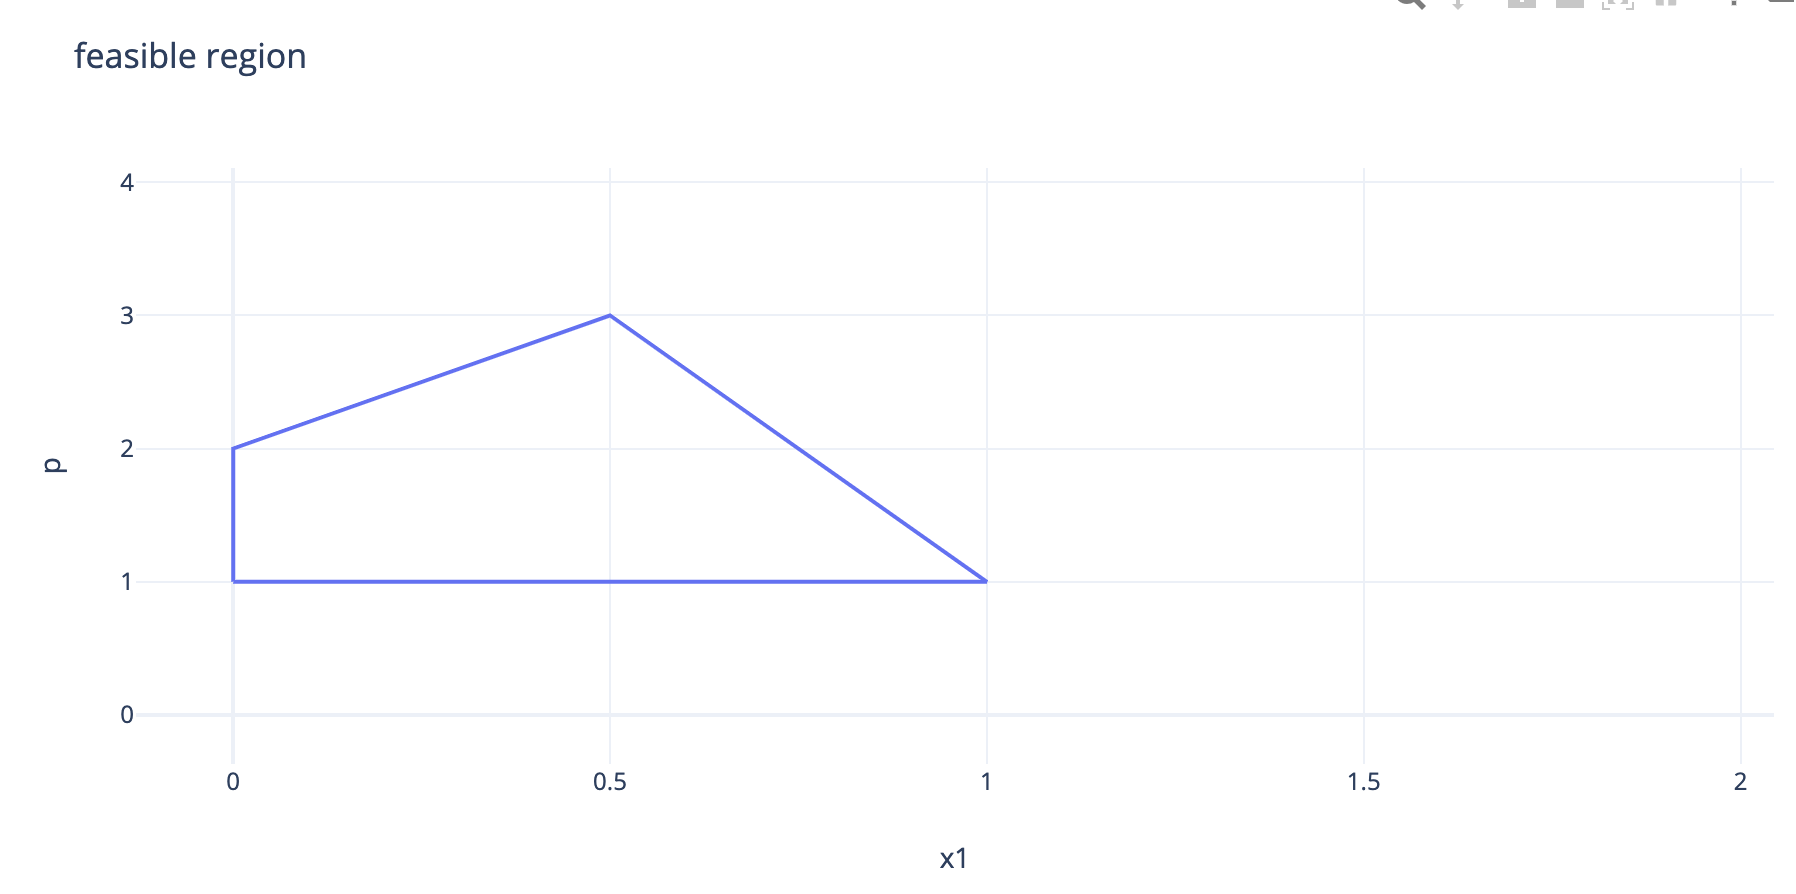
\includegraphics[width=.8\textwidth]{feasible_region.png}
	\caption{\label{fig:feasible_region}Feasible Region}
	\end{figure}
	
	\item
	
	The optimal solution is $(\frac{1}{2}, \frac{1}{2})$ and the value of game is 3.
	
\end{qparts}




\newpage
\section{Repairing a Flow}
\begin{qparts}
	\item \textbf{Main Idea}
	
	Build the residual network based on maximum flow $f$. Then find a path from $t$ to $s$ that go through edge $(v, u)$ in residual network. Push 1 unit flow into this path and fix the wrong capacity from $c_{uv}$ to $c_{uv} - 1$. Then run the original max-flow algorithm starting from this residual network.

	\item \textbf{Proof of Correctness}
	
	Pushing 1 unit back from $t$ to $s$ that go through edge $(v, u)$ will make the flow go through edge $(u, v)$ be valid. Then run the original max-flow algorithm again from this is sure will give an optimal solution.
	
	\item \textbf{Runtime Analysis}
	
	Build residual network will cost $O(|E|)$ time. Find a path from $t$ to $s$ that go through edge $(v, u)$ by DFS or BFS will cost $O(|V| + |E|)$ time. Then push 1 unit into this path will cost at most $|E|$ time. Since the max-flow solution after repairing capacity of edge $(u, v)$ cannot be larger than the original one. At most 1 iteration is needed if run max-flow algorithm starting from this. So total runtime is still linear, which is $O(|V| + |E|)$.

\end{qparts}

\newpage
\section{Generalized Max Flow}
\begin{qparts}
	\item \textbf{Constraints}
	
	\renewcommand{\theenumii}{\roman{enumii}}
	\begin{enumerate}
		\item \textbf{Capacity Constraints}
		
		\[
			\sum_{i=1}^{k} f_e^{(i)} \le c_e \text{\quad for } \forall e
		\]
		
		\item \textbf{Flow Conservation}
		
		\[
			\sum_{i=1}^{k} \sum_{u:(u, v)\in E} f_{(u, v)}^{(i)}  = \sum_{i=1}^{k} \sum_{u:(v, w)\in E} f_{(v, w)}^{(i)} \text{\quad for } \forall v \text{ except }s1, \cdots, s_k, t_1, \cdots, t_k
		\]
		
		\item \textbf{Nonnegativity}
		
		\[
			 f_e^{(i)} \ge 0 \text{\quad for } \forall e, i = 1, \cdots, k
		\]
		
		\item \textbf{Demand Constraints}
		
		\[
			\sum_{u:(u, t_i)\in E} f_{(u, t_i)}^{(i)} \ge d_i \text{\quad for }  i = 1, \cdots, k
		\]
		
	\end{enumerate}


	\item \textbf{Objective}
	
	\[
		\max \sum_{i=1}^{k}\sum_{u:(u, t_i)\in E} f_{(u, t_i)}^{(i)}
	\]
	
	The sum of all flows go to destination.


\end{qparts}

\newpage
\section{Reductions Among Flows}
\begin{qparts}
	
	\item 

	Separate each vertex into two new vertices and denote them as $v_{in}$ and $v_{out}$. Then link all incoming edges in original graph $G$ to $v_{in}$ and all outcoming edges to $v_{out}$. More formally, create a new edge $(u, v_{in})$ in new graph if edge $(u, v)$ is in original graph and create a new edge $(v_{out}, u)$ in new graph if edge $(v, u)$ is in original graph. Finally, create a new edge $(v_{in}, v_{out})$ with capacity $c_v$.
	
	Proof:
	
	If $F$ is a flow in $G$ satisfying the vertex capacity constraint, set $f_{(v_{in}, v_{out})}$ to be $\sum_{u:(u, v)\in E} f_{uv}$ and let all other flows remain same. This is a valid flow because $f_{(v_{in}, v_{out})} = \sum_{u:(u, v)\in E} f_{uv} \le c_v$. And since all other flows are unchanged, it's flow with same size.
	
	If $F\prime$ is a flow in $G\prime$, ignore all $f_{(v_{in}, v_{out})}$ will give a valid flow $F$ in $G$ with same size.

	\item 

	Create an artificial vertex $s$ and create edges $(s, s_1), \cdots, (s, s_k)$ with $\infty$ capacity.
	
	Proof:
	
	If $F$ is a flow in $G$ satisfying the vertex capacity constraint, there's always a possible solution in $G\prime$ with same size. Since the capacity for edges $(s, s_1), \cdots, (s, s_k)$ is infinity. It can be arbitrary large. So just assign $f_{(s, s_i)}$ with $\sum_{w:(s_i, w) \in E}f_{(s_i, w)}$.
	
	If $F\prime$ is a flow in $G\prime$, ignore all $f_{(s, s_i)}$ will give a valid flow $F$ in $G$ with same size.	
		
\end{qparts}
\newpage
\section{A Flowy Metric}
\begin{qparts}
	
	\item 

	According to \textbf{Max-flow min-cut theorem}, the size of the maximum flow in a network equals the capacity of the smallest $(s, t)$-cut. Since any cut in G has capacity at least 1, the max flow from $s$ to $t$ is at least 1.
	
	\item
		
\end{qparts}








\end{document}